\begin{frame}{LEF: a master and its placement boundary}
\slidesource{\href{https://github.com/The-OpenROAD-Project/OpenROAD-flow-scripts/blob/master/flow/platforms/nangate45/lef/NangateOpenCellLibrary.macro.lef}{Cell LEF}}
\centering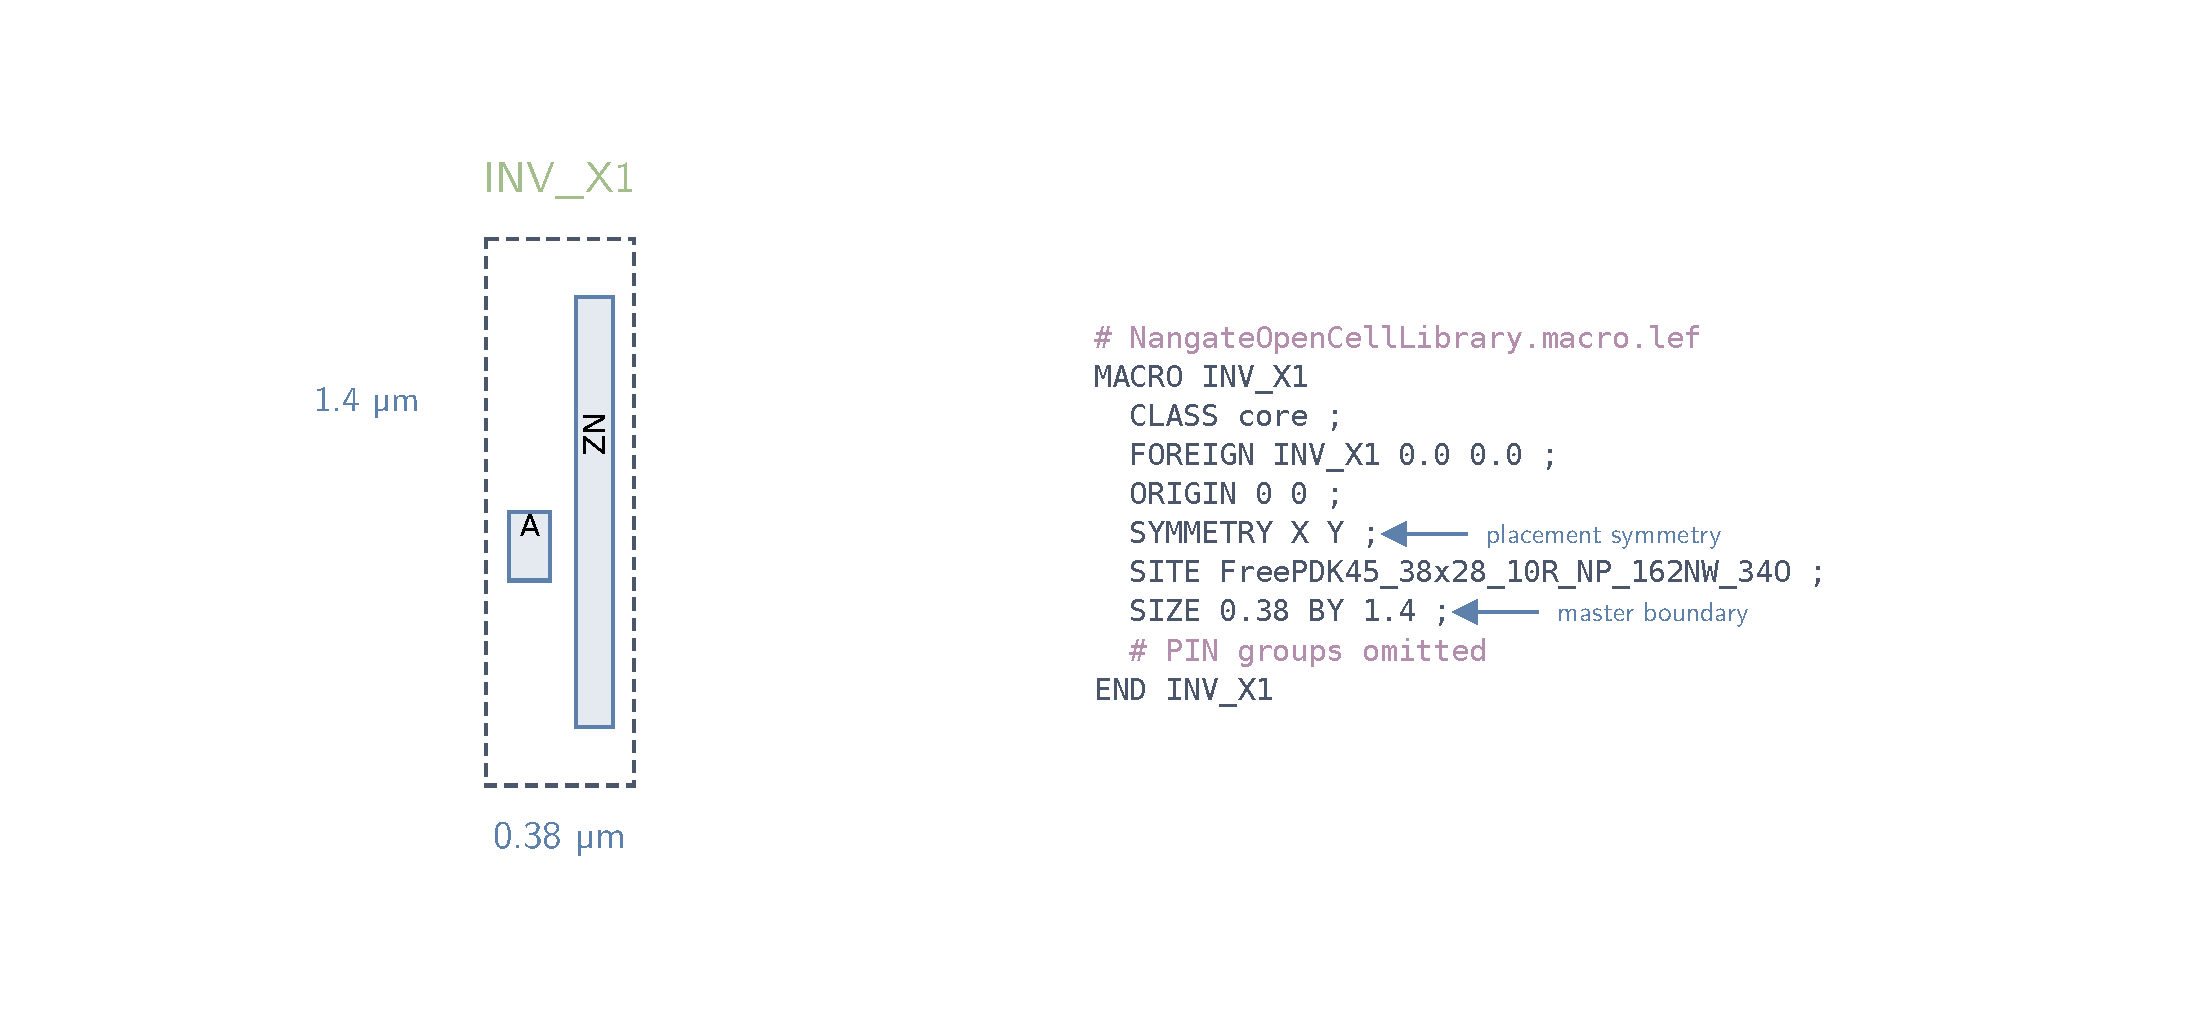
\includegraphics[width=\textwidth,height=.81\textheight,keepaspectratio]{assets/extension/lef_macro.pdf}
\note{Source excerpt retains Nangate45 values; comments mark omissions. The left diagram illustrates the highlighted quantities. Cell coordinates are in micrometers. See examples/extension for editable excerpts.}
\end{frame}

\begin{frame}{LEF: a signal pin is geometry}
\slidesource{\href{https://github.com/The-OpenROAD-Project/OpenROAD-flow-scripts/blob/master/flow/platforms/nangate45/lef/NangateOpenCellLibrary.macro.lef}{Cell LEF}}
\centering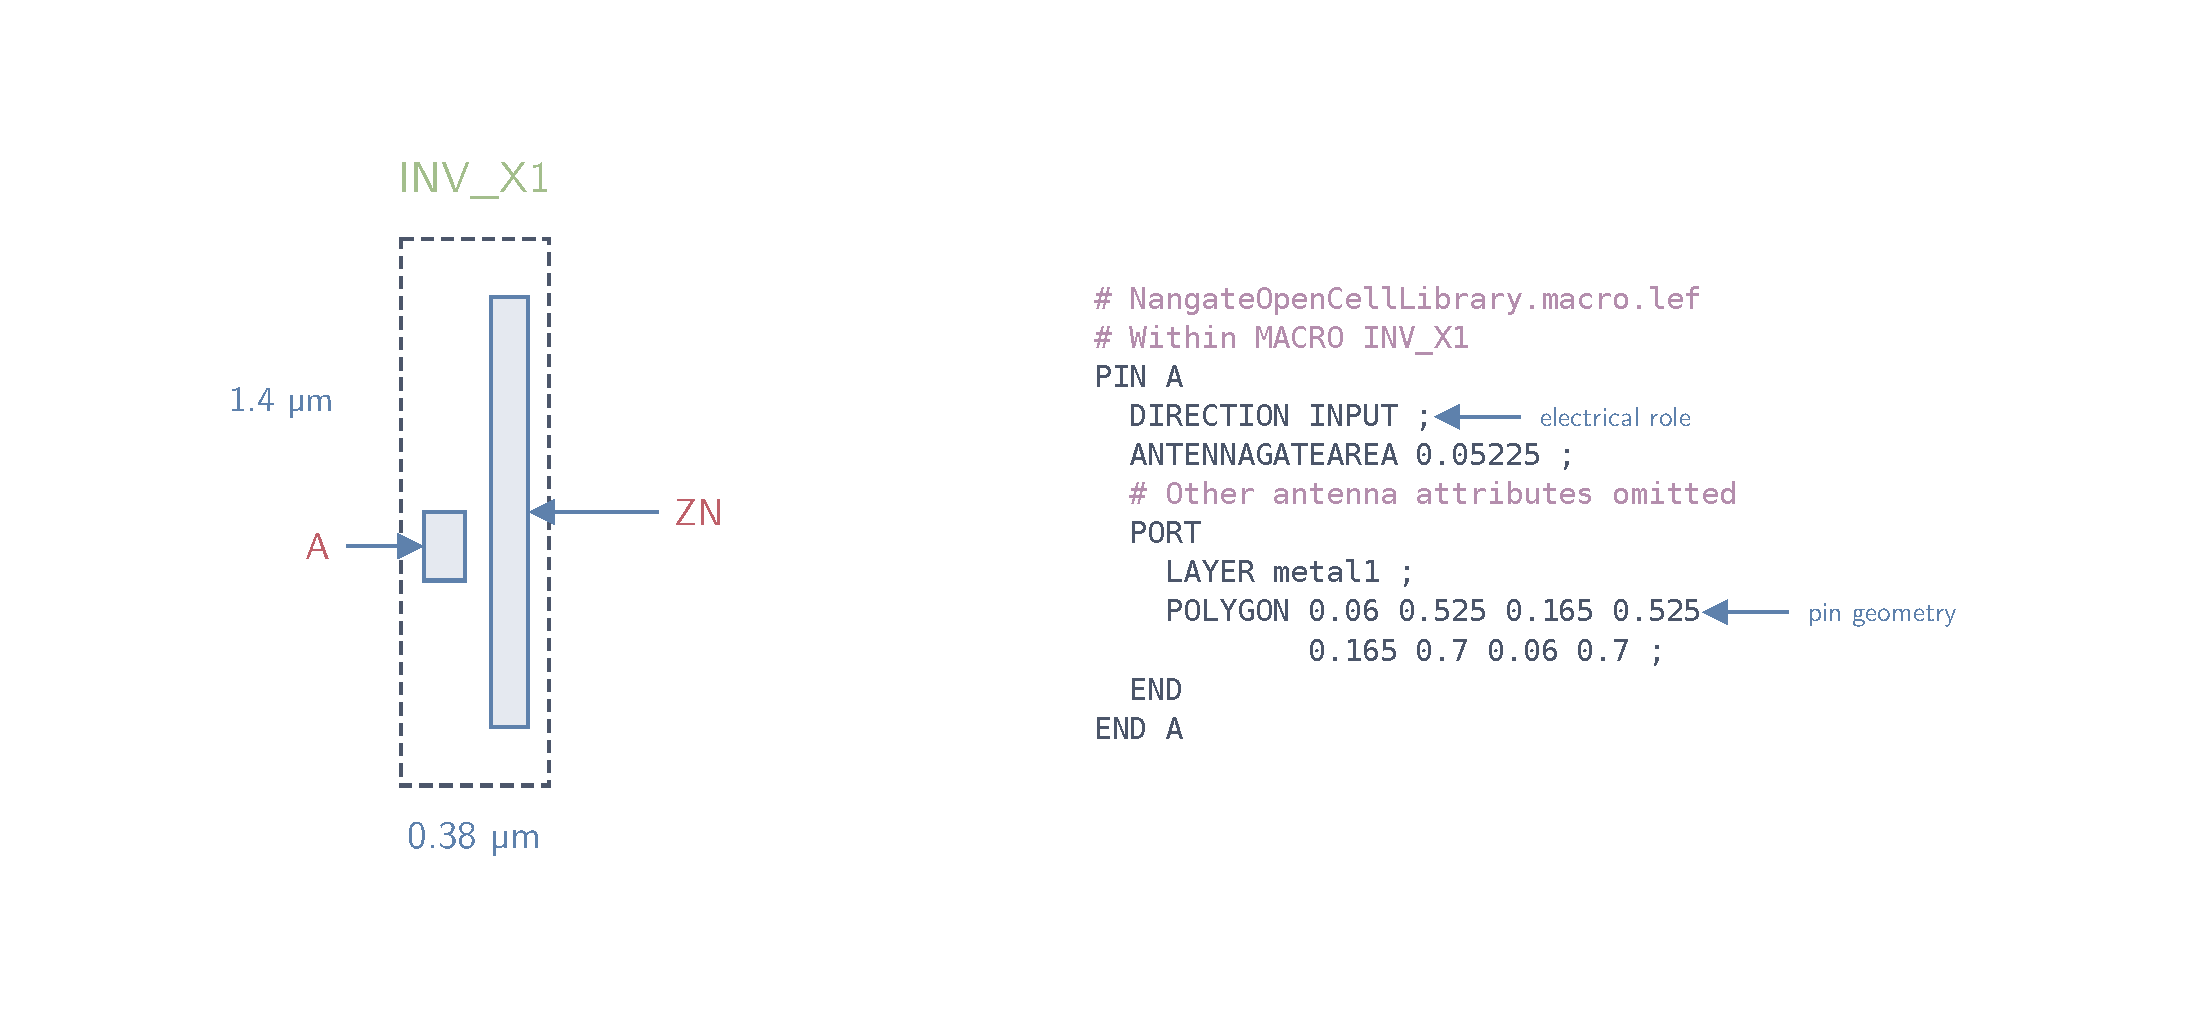
\includegraphics[width=\textwidth,height=.81\textheight,keepaspectratio]{assets/extension/lef_signal.pdf}
\note{Source excerpt retains Nangate45 values; comments mark omissions. The left diagram illustrates the highlighted quantities. Cell coordinates are in micrometers. See examples/extension for editable excerpts.}
\end{frame}

\begin{frame}{LEF: power pins and rails}
\slidesource{\href{https://github.com/The-OpenROAD-Project/OpenROAD-flow-scripts/blob/master/flow/platforms/nangate45/lef/NangateOpenCellLibrary.macro.lef}{Cell LEF}}
\centering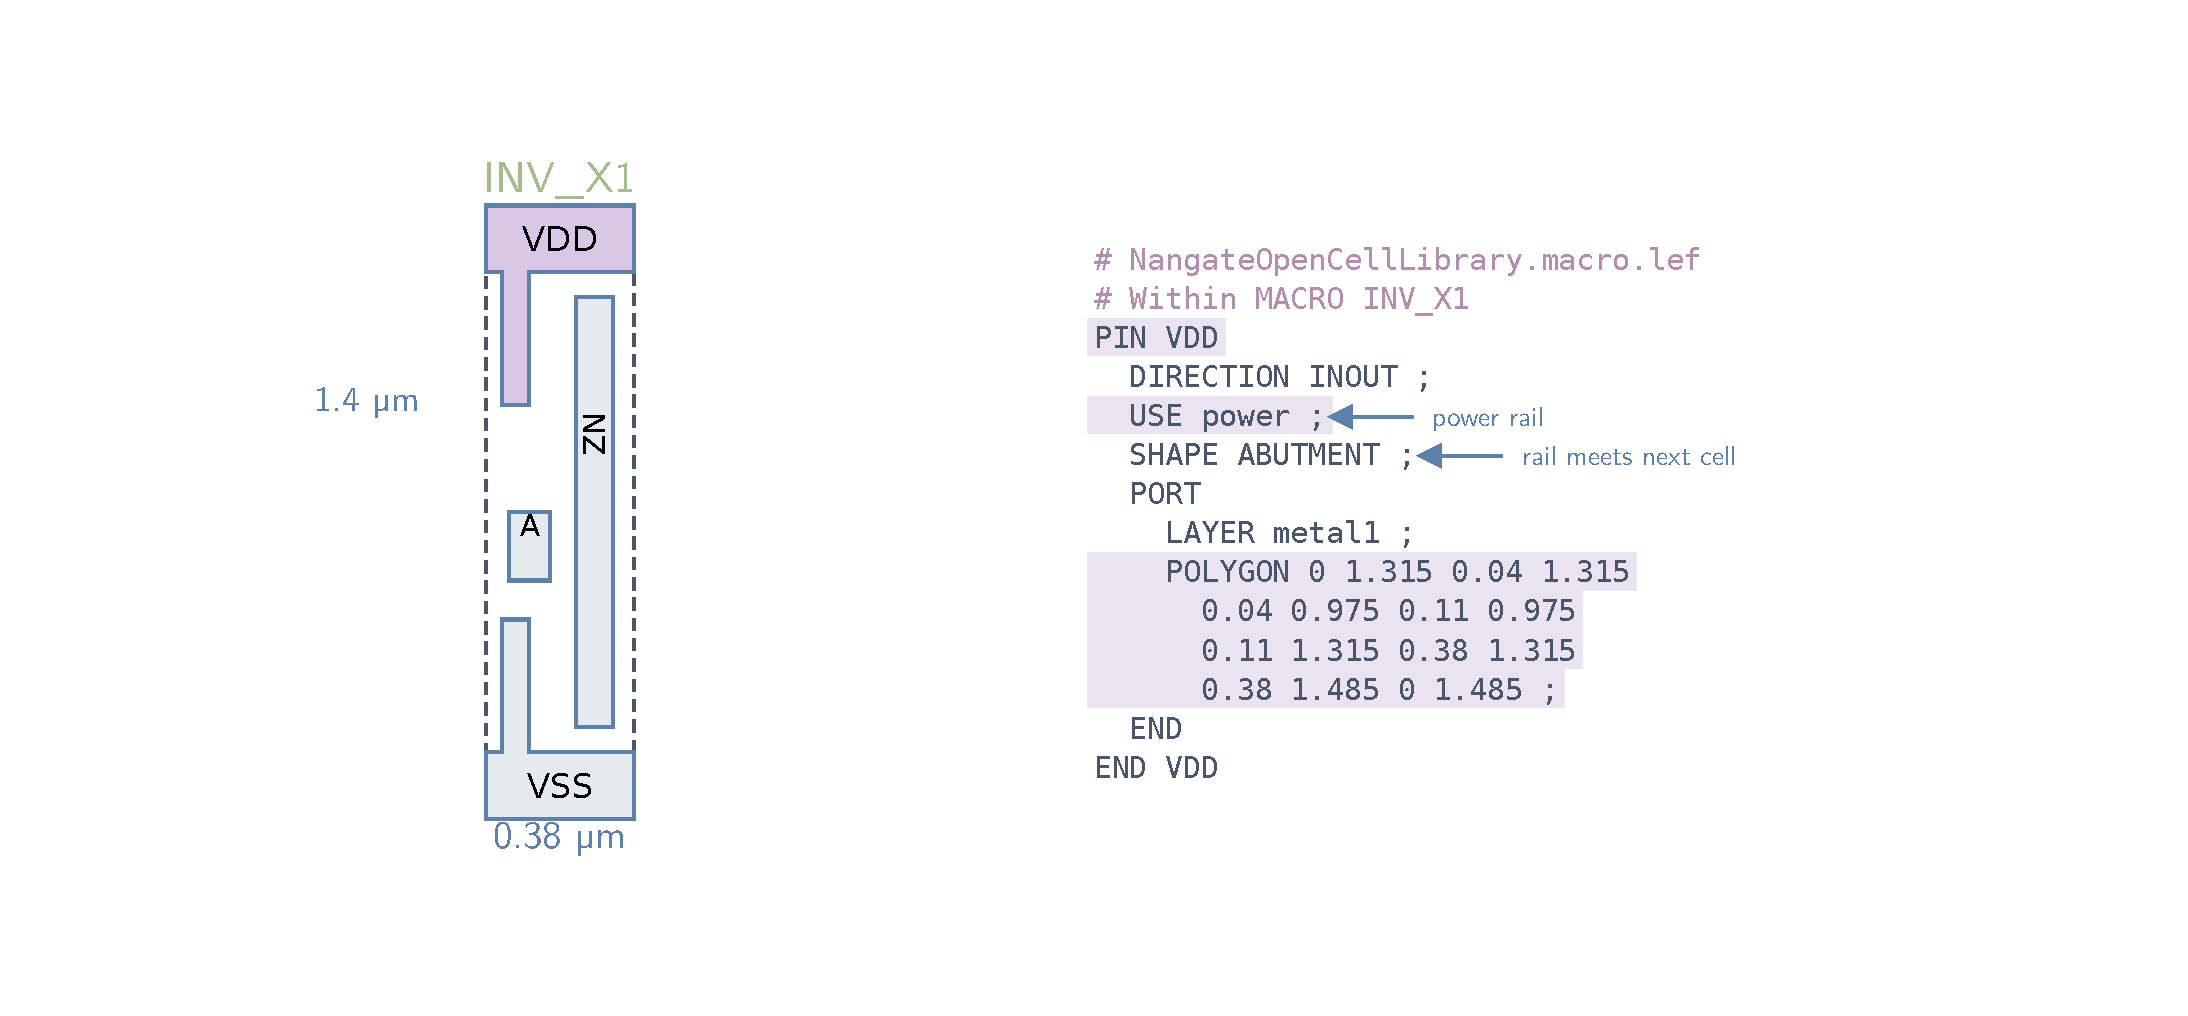
\includegraphics[width=\textwidth,height=.81\textheight,keepaspectratio]{assets/extension/lef_power.pdf}
\note{Source excerpt retains Nangate45 values; comments mark omissions. The left diagram illustrates the highlighted quantities. Cell coordinates are in micrometers. See examples/extension for editable excerpts.}
\end{frame}

\begin{frame}{LEF: units, manufacturing grid and sites}
\slidesource{\href{https://github.com/The-OpenROAD-Project/OpenROAD-flow-scripts/blob/master/flow/platforms/nangate45/lef/NangateOpenCellLibrary.tech.lef}{Tech LEF}}
\centering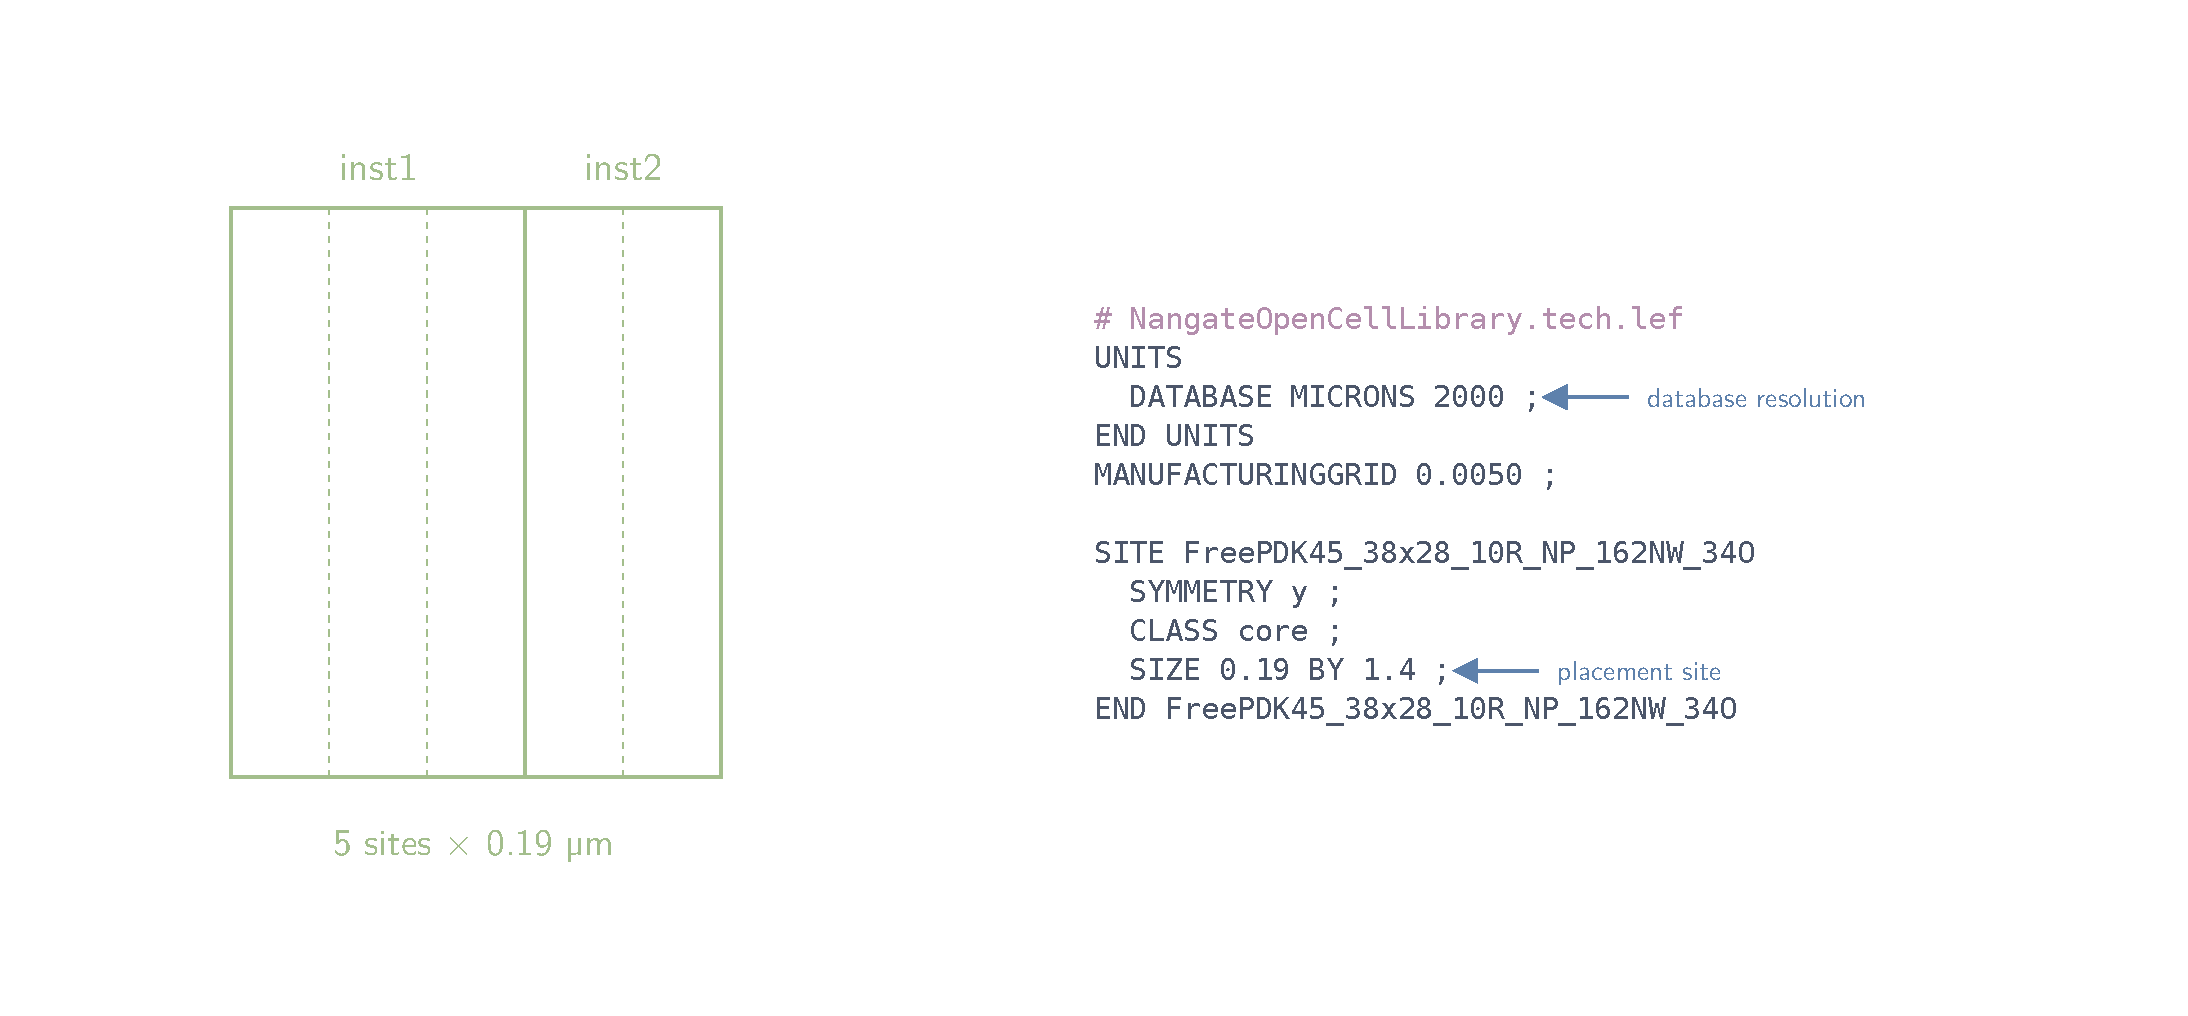
\includegraphics[width=\textwidth,height=.81\textheight,keepaspectratio]{assets/extension/lef_site.pdf}
\note{Source excerpt retains Nangate45 values; comments mark omissions. The left diagram illustrates the highlighted quantities. Cell coordinates are in micrometers. See examples/extension for editable excerpts.}
\end{frame}

\begin{frame}{LEF: a routing layer}
\slidesource{\href{https://github.com/The-OpenROAD-Project/OpenROAD-flow-scripts/blob/master/flow/platforms/nangate45/lef/NangateOpenCellLibrary.tech.lef}{Tech LEF}}
\centering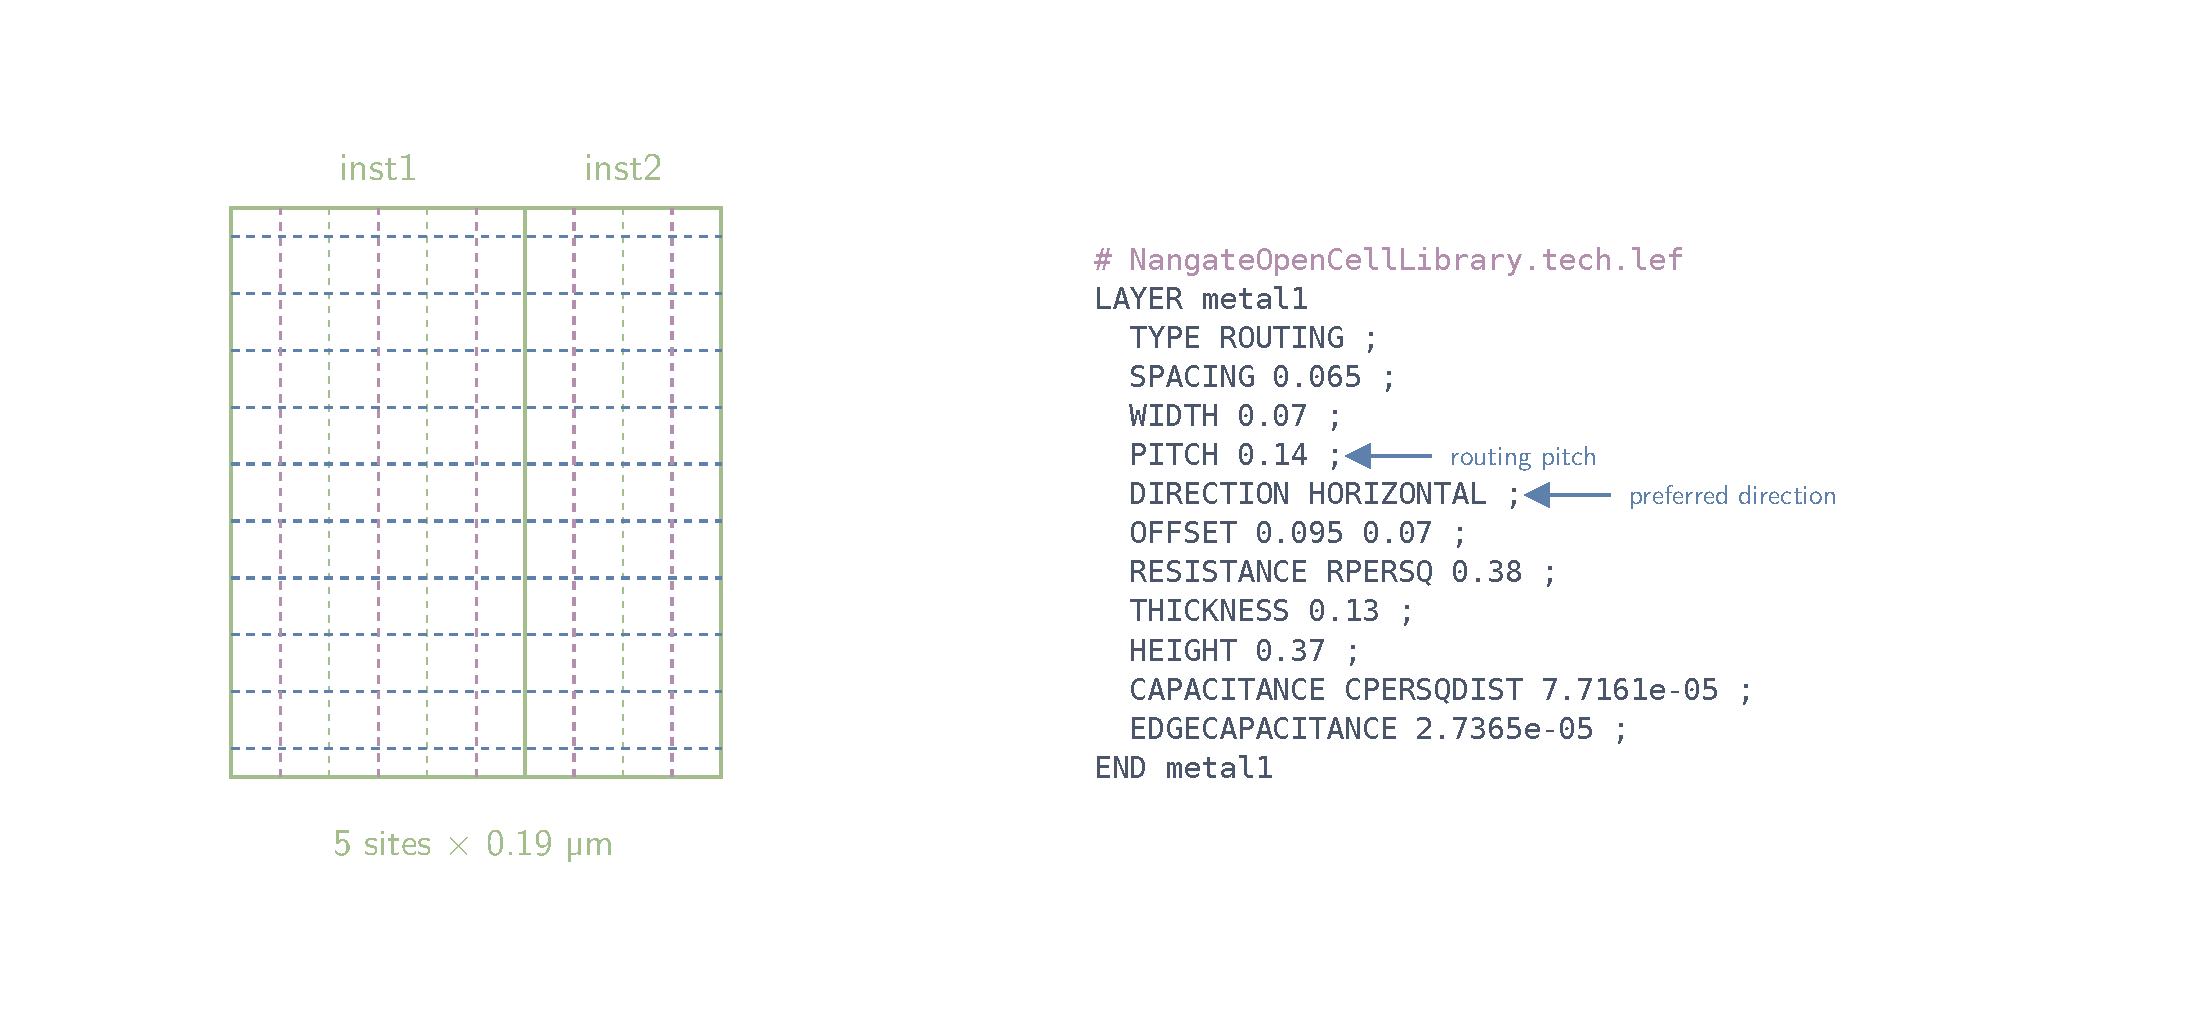
\includegraphics[width=\textwidth,height=.81\textheight,keepaspectratio]{assets/extension/lef_layer.pdf}
\note{Source excerpt retains Nangate45 values; comments mark omissions. The left diagram illustrates the highlighted quantities. Cell coordinates are in micrometers. See examples/extension for editable excerpts.}
\end{frame}

\begin{frame}{LEF: crossing between metal layers}
\slidesource{\href{https://github.com/The-OpenROAD-Project/OpenROAD-flow-scripts/blob/master/flow/platforms/nangate45/lef/NangateOpenCellLibrary.tech.lef}{Tech LEF}}
\centering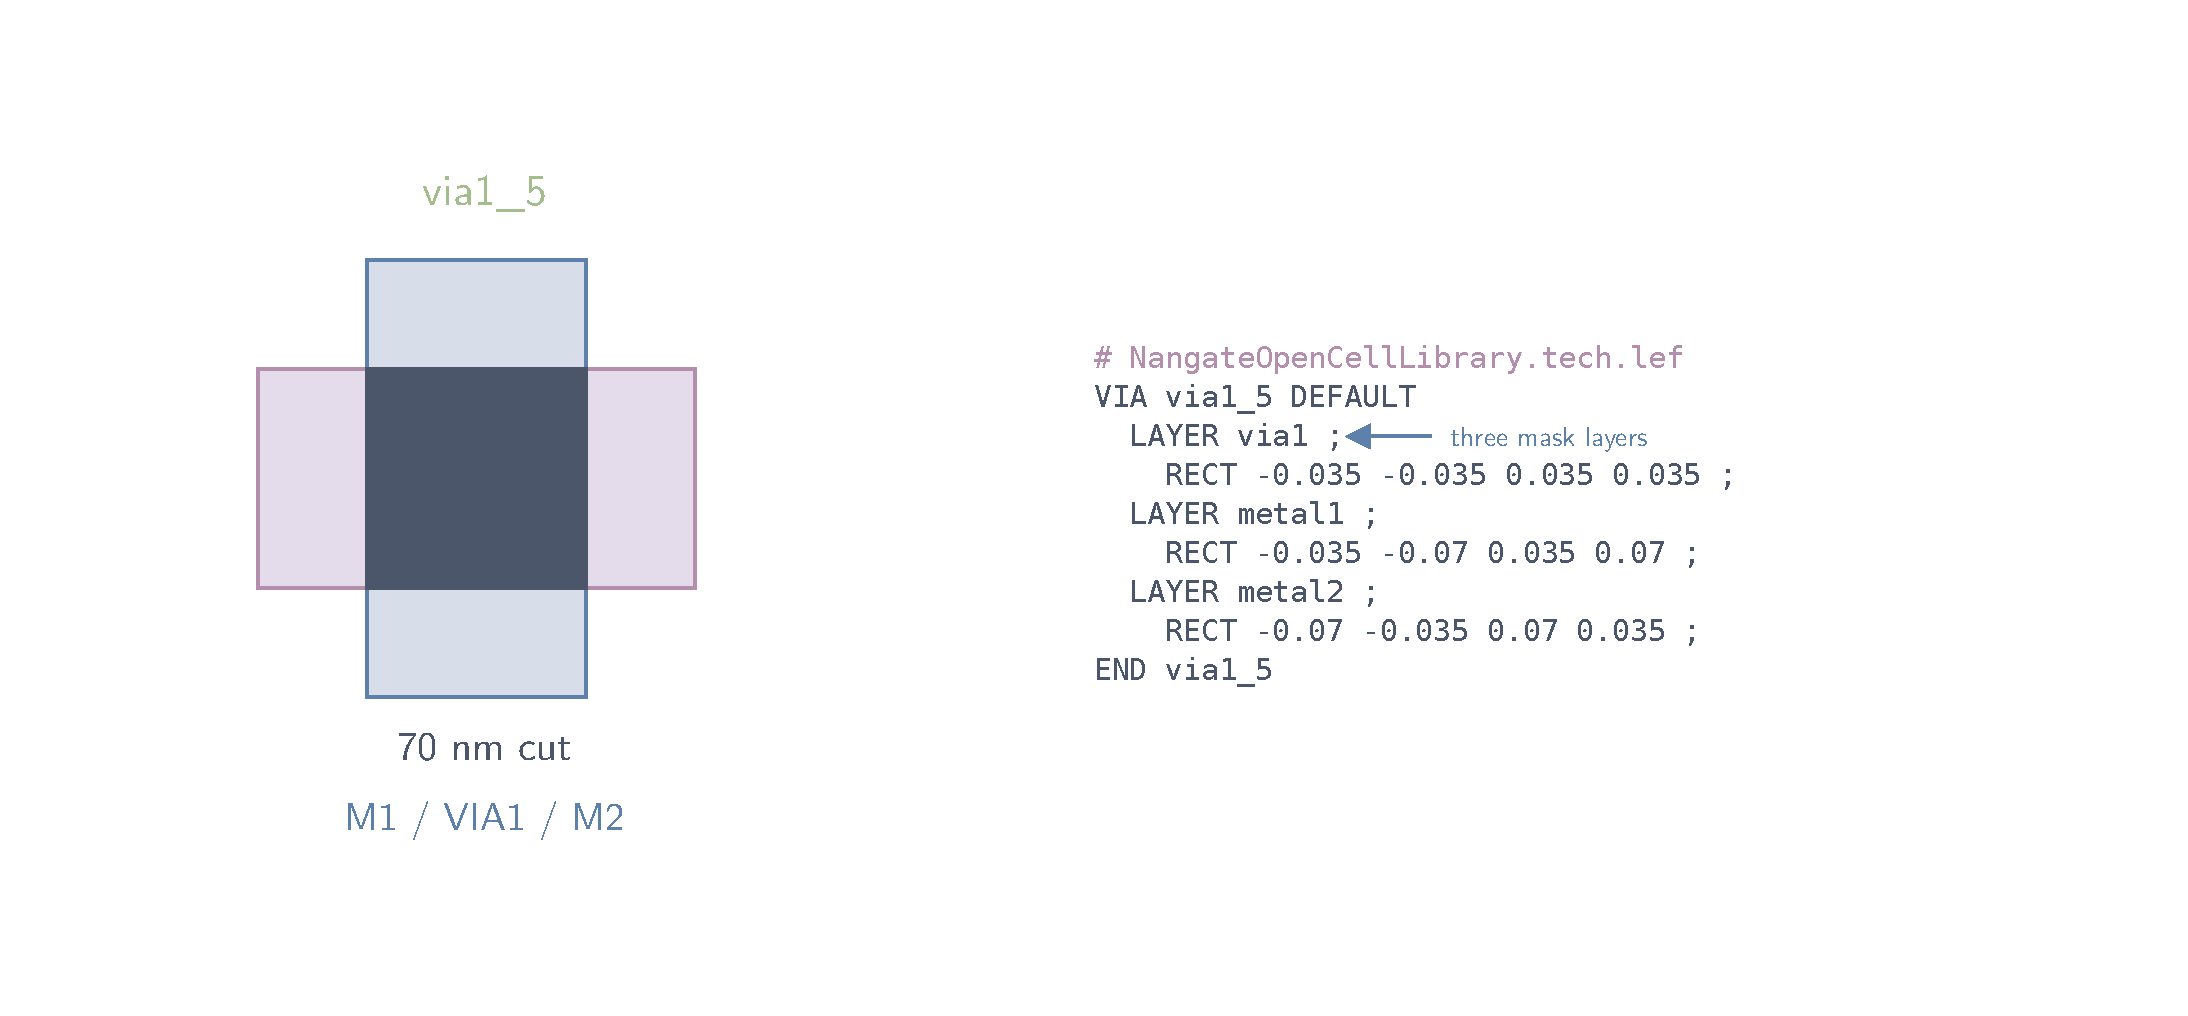
\includegraphics[width=\textwidth,height=.81\textheight,keepaspectratio]{assets/extension/lef_via.pdf}
\note{Source excerpt retains Nangate45 values; comments mark omissions. The left diagram illustrates the highlighted quantities. Cell coordinates are in micrometers. See examples/extension for editable excerpts.}
\end{frame}

\section[Timing and Power]{Timing and Power (Liberty)}

\begin{frame}{One inverter, with real input and output loading}
\slidesource{\href{https://github.com/The-OpenROAD-Project/OpenROAD-flow-scripts/blob/master/flow/platforms/nangate45/cdl/NangateOpenCellLibrary.cdl}{Cell SPICE}\enspace\textperiodcentered\enspace\href{https://ngspice.sourceforge.io/}{ngspice}}
\centering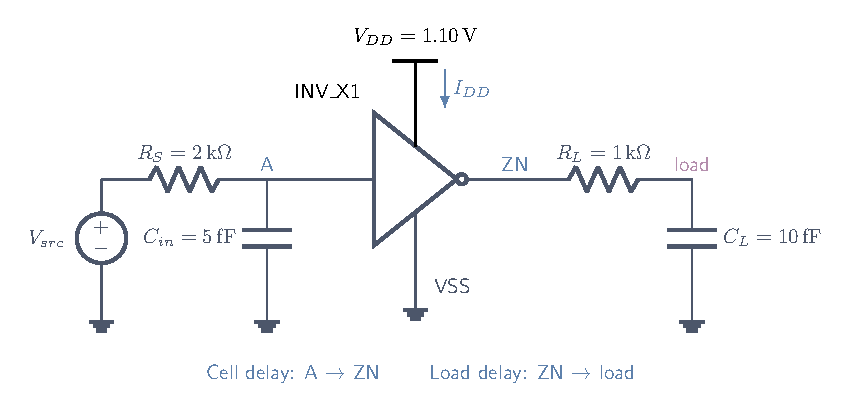
\includegraphics[width=.96\textwidth,height=.77\textheight,keepaspectratio]{assets/loaded-inverter.pdf}
\note{ngspice 45.2, real INV_X1 CDL dimensions, FreePDK45 nominal NMOS_VTL and PMOS_VTL BSIM4 cards adapted for ngspice. 1.1 V, 25 degrees C. Input 2 kilohms and 5 fF; output 1 kilohm and 10 fF. No extracted parasitics. This is an illustrative transient experiment, not reproduction of library characterization. Full executable deck: simulation/inverter_test.sp.}
\end{frame}

\begin{frame}{Propagation delay: input 50\% to output 50\%}
\slidesource{\href{https://github.com/The-OpenROAD-Project/OpenROAD-flow-scripts/blob/master/flow/platforms/nangate45/cdl/NangateOpenCellLibrary.cdl}{Cell SPICE}\enspace\textperiodcentered\enspace\href{https://ngspice.sourceforge.io/}{ngspice}}
\centering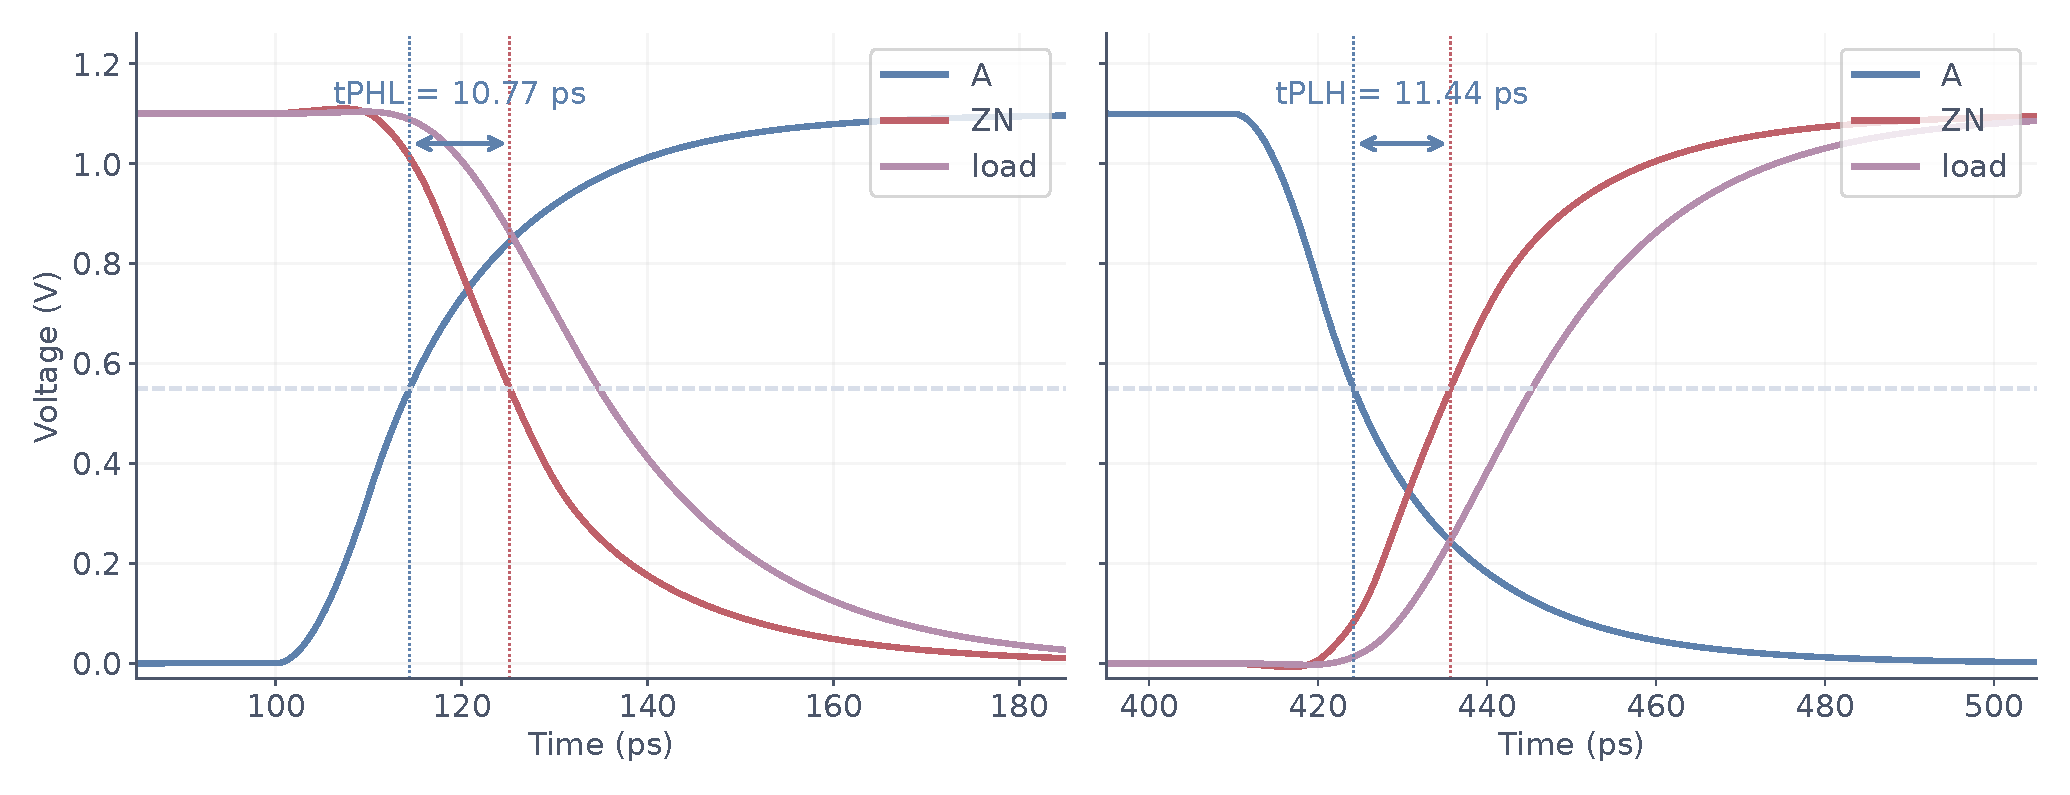
\includegraphics[width=\textwidth,height=.81\textheight,keepaspectratio]{assets/extension/propagation.pdf}
\note{Measured at cell pins A and ZN. Purple is the separate load node after the output resistor, not the cell output used for cell-delay measurement. tPHL=10.773 ps, tPLH=11.443 ps. These values depend on the chosen stimulus and RC load.}
\end{frame}

\begin{frame}{Slew: how long does the transition take?}
\slidesource{\href{https://github.com/The-OpenROAD-Project/OpenROAD-flow-scripts/blob/master/flow/platforms/nangate45/lib/NangateOpenCellLibrary_typical.lib}{Liberty}\enspace\textperiodcentered\enspace\href{https://ngspice.sourceforge.io/}{ngspice}}
\centering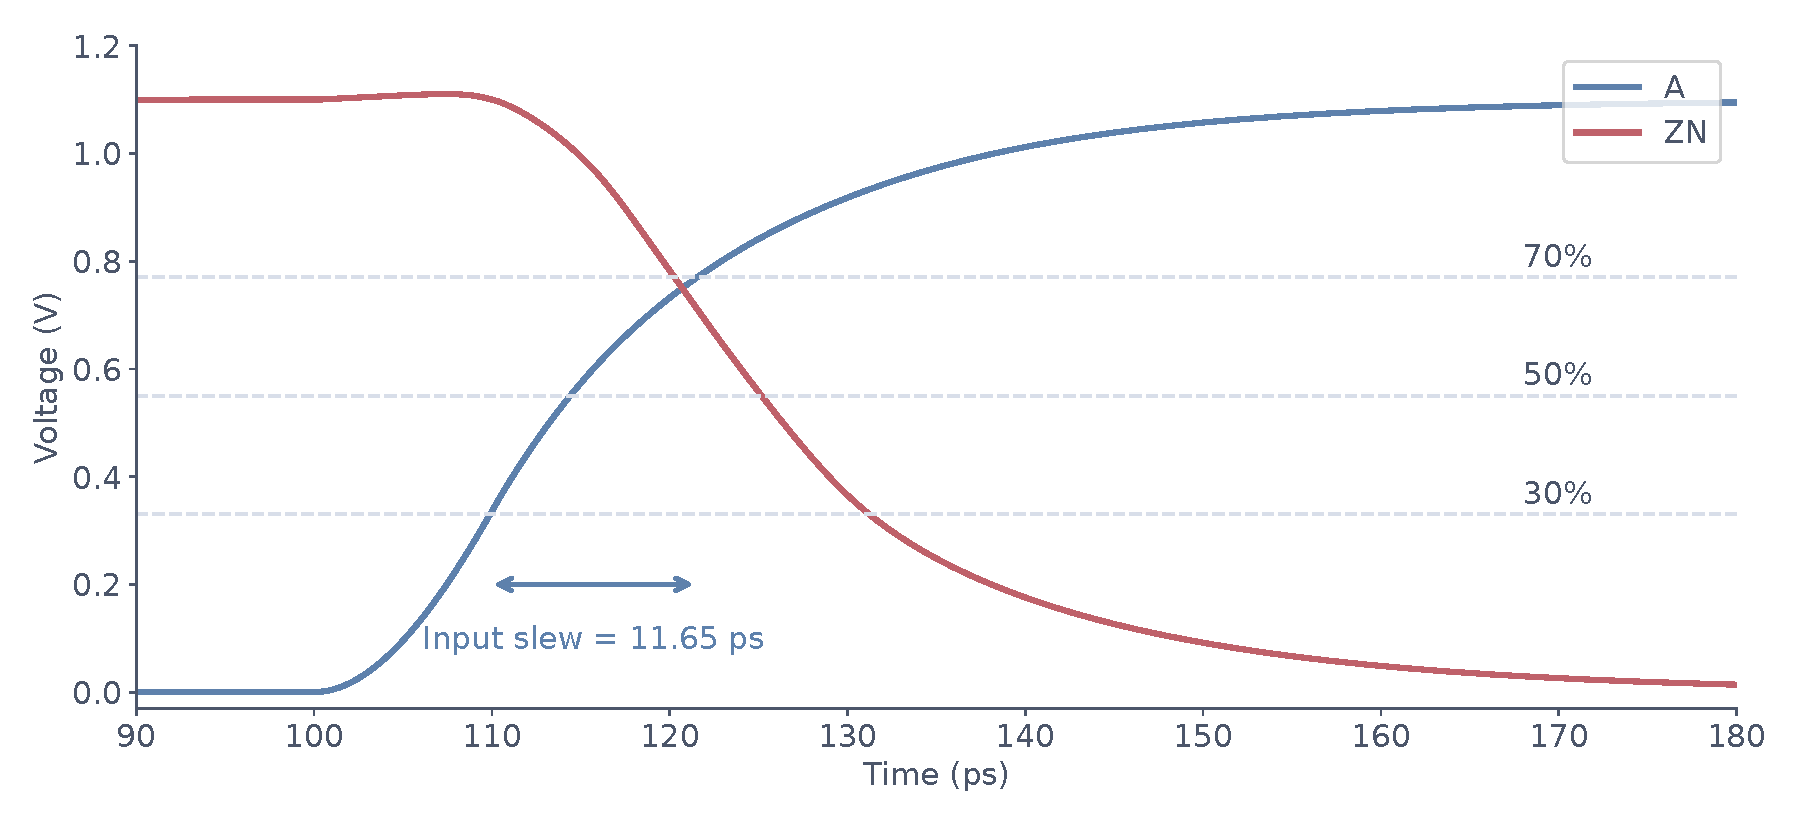
\includegraphics[width=\textwidth,height=.81\textheight,keepaspectratio]{assets/extension/slew.pdf}
\note{Nangate45 Liberty defines slew at 30 and 70 percent of the supply, and delay at 50 percent. Measured input rise slew is 11.645 ps.}
\end{frame}

\begin{frame}{Power: energy drawn from the supply}
\slidesource{\href{https://github.com/The-OpenROAD-Project/OpenROAD-flow-scripts/blob/master/flow/platforms/nangate45/cdl/NangateOpenCellLibrary.cdl}{Cell SPICE}\enspace\textperiodcentered\enspace\href{https://ngspice.sourceforge.io/}{ngspice}}
\centering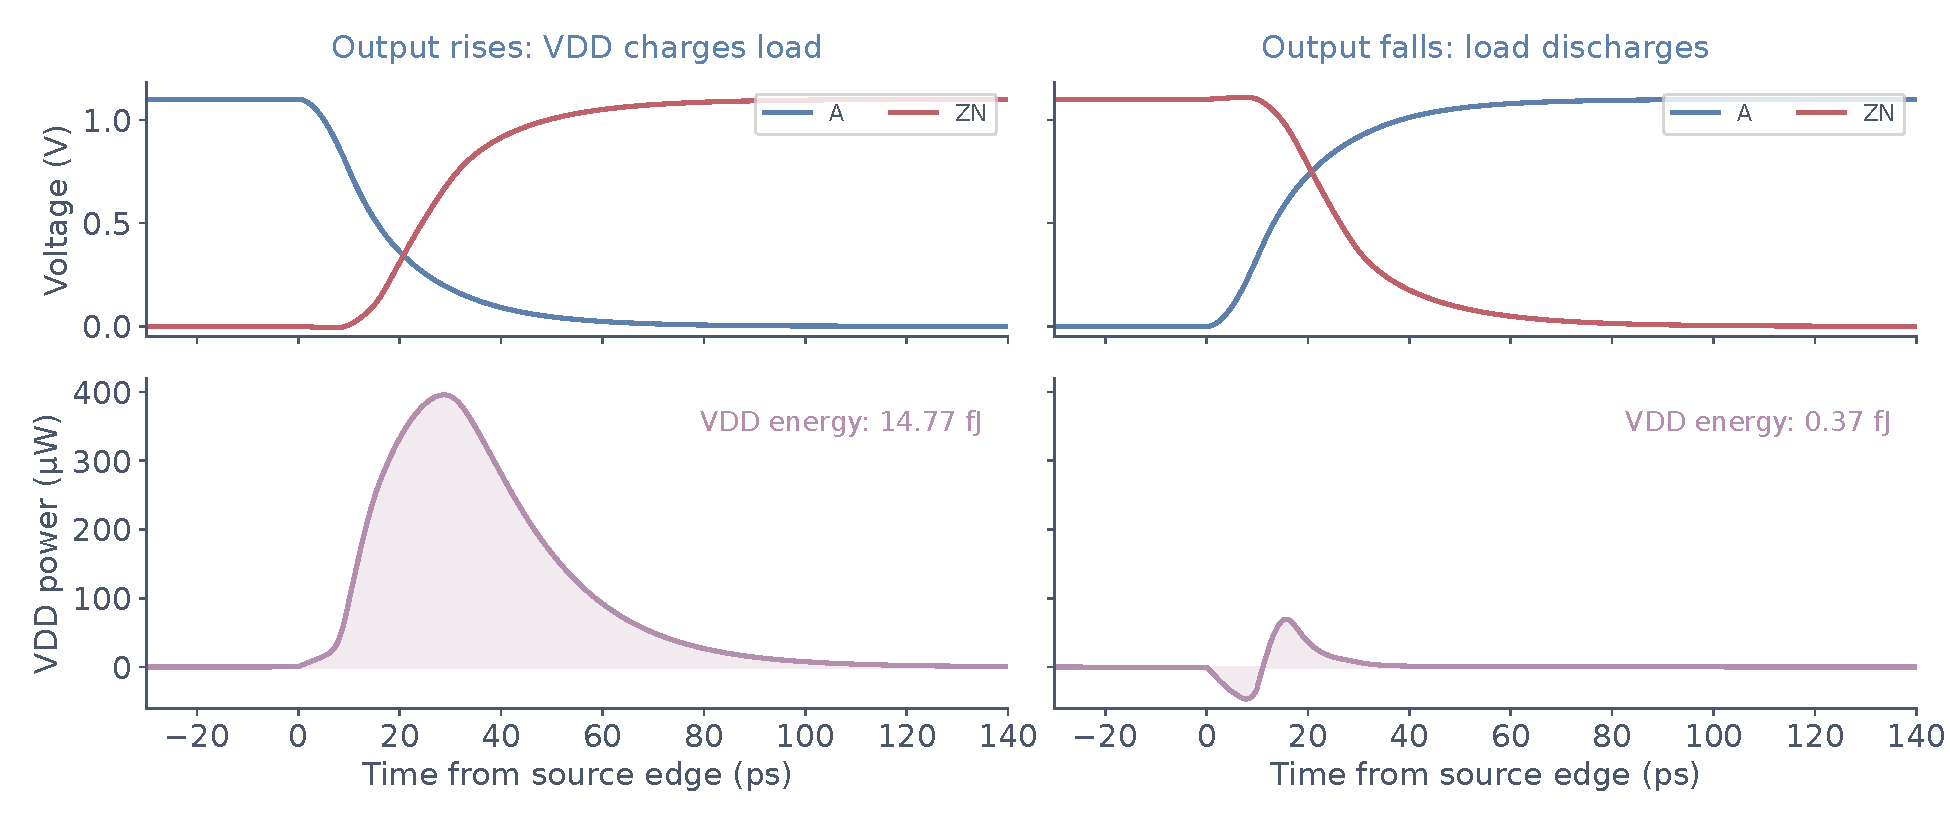
\includegraphics[width=\textwidth,height=.81\textheight,keepaspectratio]{assets/extension/power.pdf}
\note{Supply power is minus V(vdd) times current through VDD. Integral over 700 to 1400 ps is 15.136 fJ per full cycle, with our external load. The left panel shows VDD charging the load (output rising); the right panel shows output discharge (output falling). The two panels have identical scales and are aligned to their respective source edges. Energy integrates the full half-cycle windows 700--1050 ps and 1050--1400 ps: 0.370 fJ for output falling and 14.766 fJ for output rising. VDD charges the capacitor during the output rise; during output fall the stored capacitor energy is released through the pull-down network. Supply power is not the same as instantaneous heat dissipated in the devices. Brief negative power indicates energy returned to the ideal supply. It includes load charging, internal switching and leakage; it is not the Liberty internal_power value. Dynamic power depends on activity and frequency.}
\end{frame}

\begin{frame}{Liberty: characterize the cell once}
\slidesource{\href{https://en.wikipedia.org/wiki/Standard_cell}{Wikipedia}\enspace\textperiodcentered\enspace\href{https://github.com/The-OpenROAD-Project/OpenROAD-flow-scripts/blob/master/flow/platforms/nangate45/lib/NangateOpenCellLibrary_typical.lib}{Liberty}}
\begin{columns}[c,onlytextwidth]\begin{column}{.48\textwidth}\centering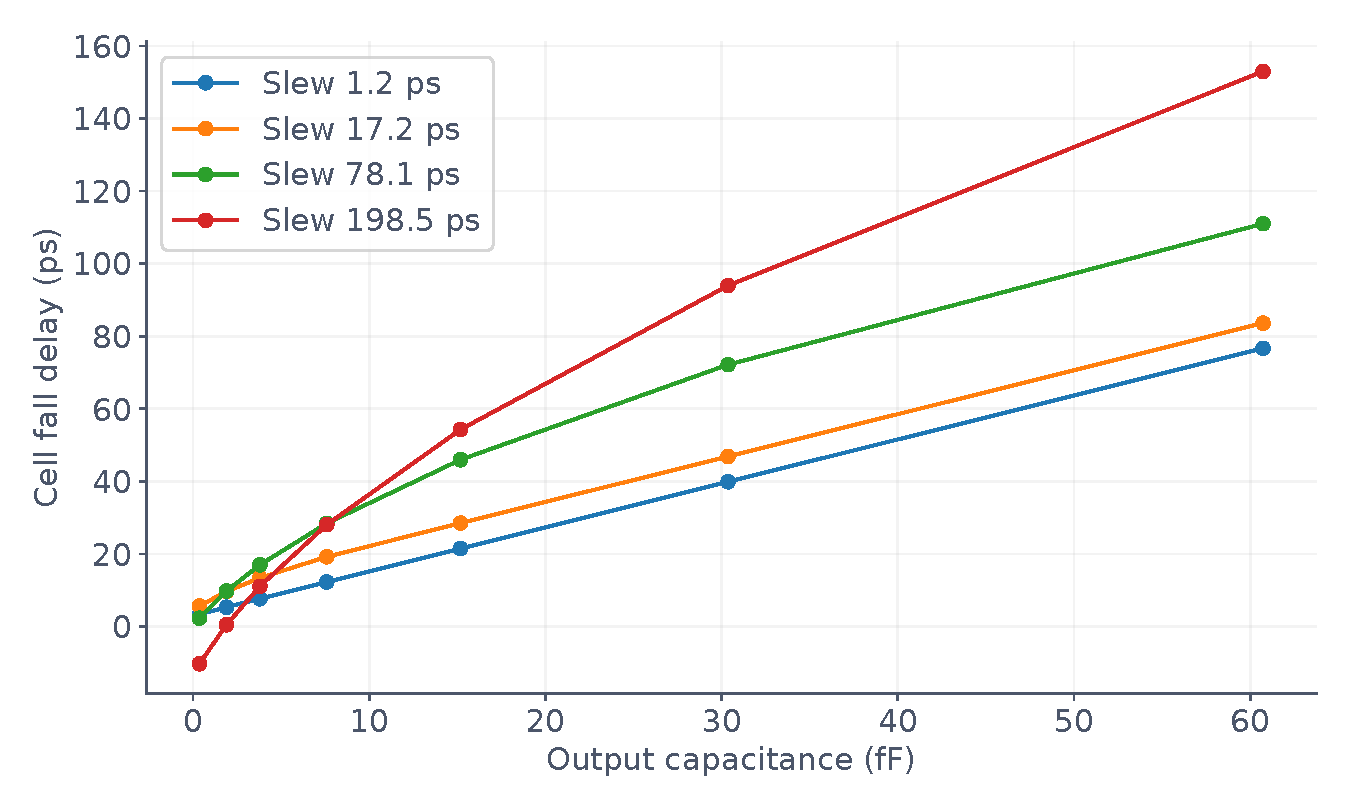
\includegraphics[width=\linewidth,height=.73\textheight,keepaspectratio]{assets/extension/liberty_table.pdf}\end{column}\begin{column}{.48\textwidth}
{\Large\textcolor{NordBlue}{Liberty (.lib)}}\\[16pt]Developed by Synopsys\\An industry library standard\\[20pt]{\large Logic, timing and power for analysis tools}\end{column}\end{columns}
\note{Liberty is a name, not an expanded acronym. Wikipedia has no dedicated Liberty-format article; the link is the related standard-cell page. Primary specification publisher: Synopsys. Plot is the actual Nangate45 INV_X1 cell_fall table, not the preceding transient experiment.}
\end{frame}

\begin{frame}{Three generations of Liberty files}
\slidesource{\href{https://www.synopsys.com/blogs/chip-design/library-characterization-for-advanced-process-designs.html}{Liberty models}}
\begin{columns}[T,onlytextwidth]
\begin{column}{.31\textwidth}
{\large\textcolor{NordBlue}{\underline{NLDM}}}\\[12pt]
\begin{itemize}\setlength{\itemsep}{7pt}
\item Simplest model: what we just showed
\item Delay and slew tables
\item Indexed by input slew and output load
\end{itemize}\vspace{10pt}
{\ttfamily\footnotesize cell\_rise / cell\_fall}
\end{column}
\begin{column}{.31\textwidth}
{\large\textcolor{NordBlue}{\underline{CCS / ECSM}}}\\[12pt]
\begin{itemize}\setlength{\itemsep}{7pt}
\item Current-waveform models
\item Capture waveform shape and load response
\item More detailed nominal timing
\end{itemize}\vspace{10pt}
{\ttfamily\footnotesize output\_current\_rise\\output\_current\_fall}
\end{column}
\begin{column}{.31\textwidth}
{\large\textcolor{NordBlue}{\underline{LVF}}}\\[12pt]
\begin{itemize}\setlength{\itemsep}{7pt}
\item Statistical variation data
\item Describe variation in delay and slew
\item Add to nominal timing models
\end{itemize}\vspace{10pt}
{\ttfamily\footnotesize ocv\_sigma\_cell\_rise\\ocv\_sigma\_cell\_fall}
\end{column}
\end{columns}
\note{Generations is used as a teaching shorthand for the evolution of library modeling, not mutually exclusive file-format versions. A Liberty file can contain NLDM tables, current-source models such as CCS, and LVF variation data. CCS/ECSM provide richer nominal behavior; LVF describes statistical variation rather than simply replacing the nominal model with a more accurate one. output_current_rise/fall are CCS keywords, not generic ECSM syntax. The Nangate45 example uses NLDM.}
\end{frame}
